\documentclass[mathserif,11pt,handout]{beamer}

\usepackage{url,verbatim,natbib}
\usepackage[english]{babel}
\usepackage{amsmath, mathabx}
\usepackage{dsfont}
\usepackage{tikz}
\usepackage{xparse}
\usepackage{pgfpages}
\pgfpagesuselayout{4 on 1}[a4paper, border shrink=5mm, landscape]

\usepackage[headheight=22pt]{beamerthemeboxes}
\usepackage{graphicx}
\beamertemplatenavigationsymbolsempty 
\setbeamercovered{transparent}
\usepackage{centernot}

\setbeamertemplate{itemize item}{$\bullet$} 
\setbeamercolor{title}{fg=uio}
\setbeamertemplate{sections/subsections in toc}[ball unnumbered]
\setbeamercolor{section in toc}{fg=uio,bg=white}
\setbeamercolor{subsection in toc}{fg=uio,bg=white}
\setbeamercolor{result}{fg=black, bg=yellow}
\newcommand{\dotsim}{\stackrel{\cdot}{\sim}}
\newcommand{\interi}{{\rm Z}\negthinspace\negthinspace {\rm Z}}
\newcommand{\reali}{{\rm I}\negthinspace {\rm R}}
\newcommand{\naturali}{{\rm I}\negthinspace {\rm N}}
\newcommand{\sign}{\mathop{\rm sgn}\nolimits}
\newcommand{\sgn}{\mathop{\mathrm{sgn}}}
\definecolor{redve}{rgb}{0.604,0.008,0.00}
\definecolor{lmu}{rgb}{0.188,0.522,0.306}
\definecolor{uio}{rgb}{0.847,0.118,0.02}

\def\R{{\rm I\!R}}
\def\P{{\rm Pr}}
\def\Real{{\rm I\!R}}
\def\T{{\footnotesize {^{_{\sf T}}}}}
\def\tr{{\rm tr}}
\def\diag{{\rm diag}}

\NewDocumentCommand\DownArrow{O{2.0ex} O{black}}{%
   \mathrel{\tikz[baseline] \draw [<-, line width=0.5pt, #2] (0,0) -- ++(0,#1);}
}

\useframetitletemplate{% 
\begin{centering} 
\begin{small} \structure{\textcolor{uio} \insertframetitle {\insertframesubtitle}}
\end{small}

\end{centering} 
}

\addheadboxtemplate{\color[rgb]{1,1,1}}{\color{uio} \underline{{\hspace{5pt}\includegraphics[scale=0.06]{../../../../support/uio_logo_eng} \hspace{0.265\paperwidth}\color{black} \tiny  STK-IN4300 - Statistical Learning Methods in Data Science} \hspace{5pt}}}

%\bfseries{\insertsection}

\addfootboxtemplate{\color[rgb]{1,1,1}}{\color{black} \tiny \quad  
STK-IN4300: lecture 3
  \hfill \tiny \insertframenumber / \inserttotalframenumber \hspace{5pt}}

  
\title{STK-IN4300 \\ Statistical Learning Methods in Data Science}
\author{Riccardo De Bin} 
\institute{debin@math.uio.no} 
\date{}


\begin{document}
\setbeamercolor{bgr}{fg=black,bg=uio}

{
\setbeamertemplate{headline}{}
\frame{
\vspace{-2cm}
\begin{beamercolorbox}[sep=-2.2em,wd=5cm,colsep=0.5pt,ht=4.25ex,dp=3ex,left]{postit}
\includegraphics[scale=0.06]{../../../../support/uio_logo_eng}
\end{beamercolorbox}
\vspace{0.365cm}
\noindent\makebox[\linewidth]{\color{uio} \rule{\paperwidth}{0.4pt}}
\vspace{2.5cm}
\titlepage
}
}

\frame{\frametitle{Outline of the lecture}
\tableofcontents
}


\section{Model Assessment and Selection}

\subsection{Cross-Validation}

\frame{\frametitle{Cross-Validation: }
\framesubtitle{$k$-fold cross-validation}
The \textcolor{uio}{cross-validation} aims at estimating the \textcolor{uio}{expected test error},
$$
\text{Err} = E[L(Y,\hat{f}(X))].
$$

\begin{itemize}
\item with \textcolor{uio}{enough data}, we can \textcolor{uio}{split} them in a training and test set;
\item since usually it is not the case, we \textcolor{uio}{mimic} this split by using the limited amount of data we have,
\begin{itemize}
\item split data in \textcolor{uio}{$K$ folds} $\mathcal{F}_1, \dots, \mathcal{F}_K$, \textcolor{uio}{approximatively same size};
\item use, in turn, \textcolor{uio}{$K-1$ folds to train} the model (derive $\hat{f}^{-k}(X)$);
\item \textcolor{uio}{evaluate} the model in the \textcolor{uio}{remaining fold},
$$
CV(\hat{f}^{-k}) = \frac{1}{|\mathcal{F}_k|}\sum_{i \in \mathcal{F}_k} L(y_i, \hat{f}^{-k}(x_i))
$$
\item \textcolor{uio}{estimate the expected test error} as an average,
\end{itemize}
\end{itemize}
$$
CV(\hat{f}) = \frac{1}{K}\sum_{k = 1}^K \frac{1}{|\mathcal{F}_k|} \sum_{i \in \mathcal{F}_k} L(y_i, \hat{f}^{-k}(x_i)) \stackrel{|\mathcal{F}_k|=\frac{N}{K}}{=} \frac{1}{N} \sum_{i =1}^N L(y_i, \hat{f}^{-k}(x_i)).
$$
}


\frame{\frametitle{Cross-Validation: }
\framesubtitle{$k$-fold cross-validation}
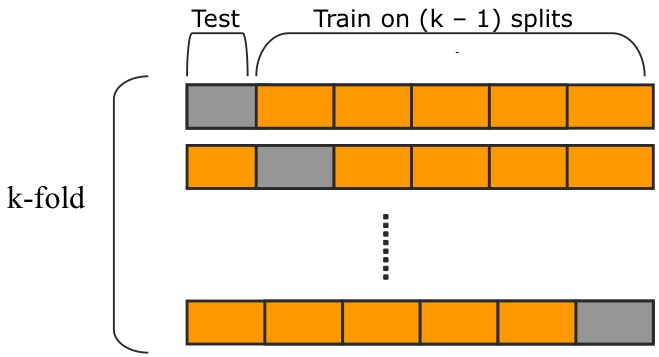
\includegraphics[width=\textwidth]{figure_cv}

\vspace{0.5cm}

{\tiny (figure from \url{http://qingkaikong.blogspot.com/2017/02/machine-learning-9-more-on-artificial.html})}
}


\frame{\frametitle{Cross-Validation: }
\framesubtitle{choice of $K$}
How to \textcolor{uio}{choose $K$}?
\begin{itemize}
\item there is \textcolor{uio}{no} a \textcolor{uio}{clear solution};
\item \textcolor{uio}{bias-variance trade-off}:
\begin{itemize}
\item smaller the $K$, smaller the variance (but larger bias);
\item larger the $K$, smaller the bias (but larger variance);
\item extreme cases:
\begin{itemize}
\item $K=2$, half observations for training, half for testing;
\item $K=N$, \textcolor{uio}{leave-one-out cross-validation} (LOOCV);
\end{itemize}
\item LOOCV estimates the expected test error \textcolor{uio}{approximatively unbiased};
\item LOOCV has very \textcolor{uio}{large variance} (the ``training sets'' are very similar to one another);
\end{itemize}
\item usual choices are $K=5$ and $K=10$.
\end{itemize}
}


\frame{\frametitle{Cross-Validation: }
\framesubtitle{choice of $K$}
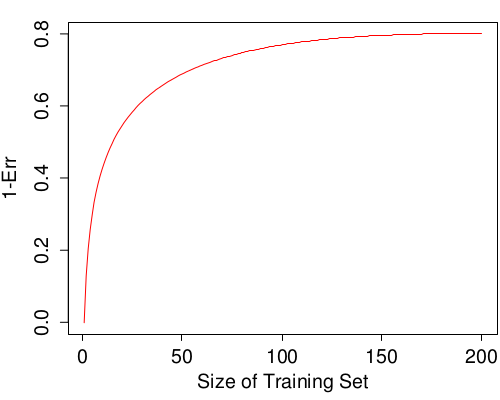
\includegraphics[width=0.9\textwidth]{error}
}


\frame{\frametitle{Cross-Validation: }
\framesubtitle{further aspects}
If we want to select a \textcolor{uio}{tuning parameter} (e.g., no. of neighbours)
\begin{itemize}
\item train $\hat{f}^{-k}(X, \alpha)$ for each $\alpha$;
\item compute $CV(\hat{f}, \alpha) = \frac{1}{K}\sum_{k = 1}^K \frac{1}{|\mathcal{F}_k|} \sum_{i \in \mathcal{F}_k} L(y_i, \hat{f}^{-k}(x_i, \alpha))$;
\item obtain $\hat{\alpha} = \text{argmin}_\alpha CV(\hat{f}, \alpha)$.
\end{itemize}

\hspace{2pt}

The \textcolor{uio}{generalized cross-validation} (GCV),
$$
GCV(\hat{f})= \frac{1}{N}\sum_{i=1}^{N} \left[ \frac{y_i - \hat{f}(x_i)}{1 - \text{trace}(S)/N} \right]^2
$$
\begin{itemize}
\item is a \textcolor{uio}{convenient approximation} of LOOCV for linear fitting under square loss;
\item has \textcolor{uio}{computational advantages}.
\end{itemize}
}


\frame{\frametitle{Cross-Validation: }
\framesubtitle{the wrong and the right way to do cross-validation}
Consider the following procedure:
\begin{enumerate}
\item find a subset of good (= most correlated with the outcome) predictors;
\item use the selected predictors to build a classifier;
\item use cross-validation to compute the prediction error.
\end{enumerate}

\hspace{2pt}

Practical example (see R file):
\begin{itemize}
\item generated $X$, an $[N=50] \times [p=5000]$ data matrix;
\item generate independently $y_i$, $i=1,\dots,50$, $y_i\in\{0,1\}$;
\item the true error test is $0.50$;
\item implementing the procedure above. What does it happen?
\end{itemize}
}

\frame{\frametitle{Cross-Validation: }
\framesubtitle{the wrong and the right way to do cross-validation}
Why it is \textcolor{uio}{not correct}?
\begin{itemize}
\item Training and test sets are \textcolor{uio}{{\bf NOT} independent}!
\item observations on the test sets are \textcolor{uio}{used twice}.
\end{itemize}

\hspace{2pt}

\textcolor{uio}{Correct} way to proceed:
\begin{itemize}
\item divide the sample in $K$ folds;
\item both perform variable selection and build the classifier \textcolor{uio}{using observations from $K-1$} folds;
\begin{itemize}
\item possible choice of the tuning parameter included;
\end{itemize}
\item compute the prediction error on the \textcolor{uio}{remaining fold}.
\end{itemize}
}


\subsection{Bootstrap Methods}

\frame{\frametitle{Bootstrap Methods: }
\framesubtitle{bootstrap}
IDEA: generate pseudo-samples from the empirical distribution function computed on the original sample;
\begin{itemize}
\item by \textcolor{uio}{sampling with replacement} from the original dataset;
\item mimic new experiments.
\end{itemize} 

\hspace{2pt}

Suppose $Z = \{\underbrace{(x_1,y_1)}_{z_1}, \dots, \underbrace{(y_N, x_N)}_{z_N}\}$ be the \textcolor{uio}{training set}:
\begin{itemize}
\item by sampling with replacement, $Z_1^* = \{\underbrace{(y_1^*,x_1^*)}_{z_1^*}, \dots, \underbrace{(y_N^*, x_N^*)}_{z_N^*}\}$;
\item \dots \hspace{20pt} \dots \hspace{20pt} \dots \hspace{20pt} \dots \hspace{20pt} \dots \hspace{20pt} \dots \hspace{20pt} \dots
\item by sampling with replacement, $Z_B^* = \{\underbrace{(y_1^*,x_1^*)}_{z_1^*}, \dots, \underbrace{(y_N^*, x_N^*)}_{z_N^*}\}$;
\item use the $B$ bootstrap samples $Z_1^*$, \dots, $Z_B^*$ to estimate \textcolor{uio}{any aspect of the distribution} of a map $S(Z)$.
\end{itemize}
}


\frame{\frametitle{Bootstrap Methods: }
\framesubtitle{bootstrap}
For example, to estimate the variance of $S(Z)$,
$$
\widehat{\text{Var}}[S(Z)] = \frac{1}{B-1}\sum_{b=1}^B (S(Z_b^*) - \bar{S^*})^2
$$
where $\bar{S^*}=\frac{1}{B}\sum_{b=1}^B S(Z_b^*)$.

\hspace{2pt}

Note that:
\begin{itemize}
\item $\widehat{\text{Var}}[S(Z)]$ is the \textcolor{uio}{Monte Carlo estimate} of $\text{Var}[S(Z)]$ under sampling from the \textcolor{uio}{empirical distribution $\hat{F}$}.
\end{itemize}
}

\frame{\frametitle{Bootstrap Methods: }
\framesubtitle{bootstrap}
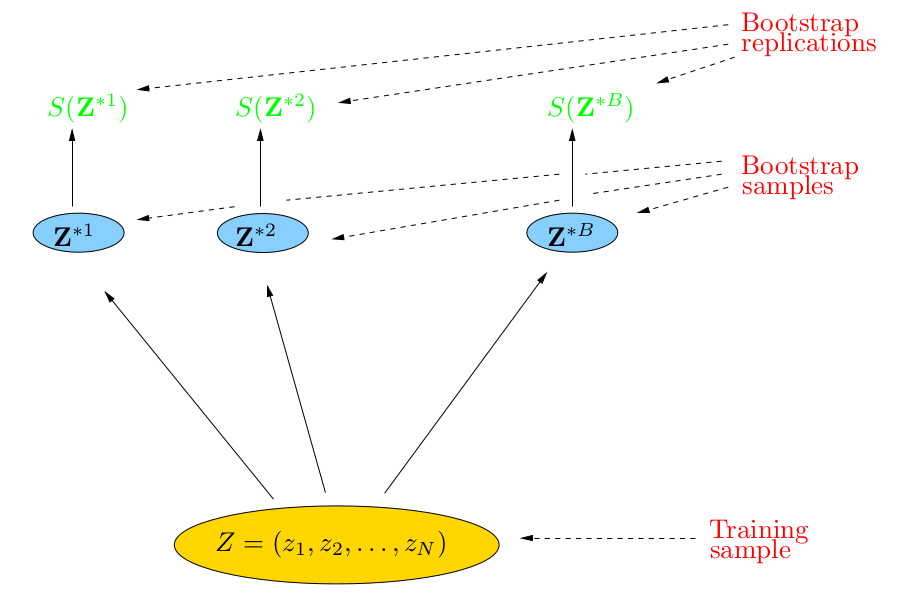
\includegraphics[width=\textwidth]{bootstrap}
}


\frame{\frametitle{Bootstrap Methods: }
\framesubtitle{estimate prediction error}
Very simple:
\begin{itemize}
\item generate $B$ bootstrap samples $Z_1^*, \dots, Z_B^*$;
\item apply the prediction rule to each bootstrap sample to derive the predictions $\hat{f}_b^*(x_i)$, $b = 1,\dots, B$;
\item compute the error for each point, and take the average,
$$
\widehat{\text{Err}}_\text{boot} = \frac{1}{B} \sum_{b=1}^B \frac{1}{N} \sum_{i=1}^N L(y_i,\hat{f}_b^*(x_i)).
$$
\end{itemize}
Is it correct? {\bf NO!!!}

\hspace{2pt}

Again, training and test set are {\bf NOT} independent!
}


\frame{\frametitle{Bootstrap Methods: }
\framesubtitle{example}
Consider a classification problem:
\begin{itemize}
\item two classes with the same number of observations;
\item predictors and class label independent $\Rightarrow$ $\text{Err} = 0.5$.
\item[]
\end{itemize}

Using the 1-nearest neighbour:
\begin{itemize}
\item if $y_i \in Z_b^* \rightarrow \hat{\text{Err}} = 0$;
\item if $y_i \notin Z_b^* \rightarrow \hat{\text{Err}} = 0.5$;
\end{itemize}
Therefore,
$$
\widehat{\text{Err}}_\text{boot} = 0 \times \P[Y_i \in Z_b^*] + 0.5 \times \underbrace{\P[Y_i \notin Z_b^*]}_{0.368} = 0.184
$$
}


\frame{\frametitle{Bootstrap Methods: }
\framesubtitle{why 0.368}
$$
\P[\text{observation } i \text{ does not belong to the boostrap sample } b] = 0.368
$$
Since
$$
\P[Z_{b[j]}^* \neq y_i] = \frac{N-1}{N},
$$
is true for each position $[j]$, then
$$
\P[Y_i \notin Z_b^*] = \left(\frac{N-1}{N}\right)^N \xrightarrow{N\rightarrow \infty} e^{-1} \approx 0.368,
$$

\hspace{2pt}

Consequently,
$$
\P[\text{observation } i \text{ is in the boostrap sample } b] \approx 0.632.
$$
}


\frame{\frametitle{Bootstrap Methods: }
\framesubtitle{correct estimate prediction error}
Note:
\begin{itemize}
\item each bootstrap sample has \textcolor{uio}{$N$ observations};
\item some of the original observations are included \textcolor{uio}{more than once};
\item some of them (in average, $0.368N$) are \textcolor{uio}{not included} at all;
\begin{itemize}
\item these are not used to compute the predictions;
\item they can be used as a \textcolor{uio}{test set},
\end{itemize}
\item[]
\end{itemize}
$$
\widehat{\text{Err}}^{(1)} = \frac{1}{N}\sum_{i=1}^N \frac{1}{|C_{[-i]}|} \sum_{b\in C_{[-i]}} L(y_i, \hat{f}_b^*(x_i))
$$
where $C_{[-i]}$ is the set of indeces of the bootstrap samples which \textcolor{uio}{do not contain} the observation $i$ and $|C_{[-i]}|$ denotes its cardinality.
}


\frame{\frametitle{Bootstrap Methods: }
\framesubtitle{0.632 bootstrap}
Issue:
\begin{itemize}
\item the \textcolor{uio}{average number of unique observations} in the bootstrap sample is \textcolor{uio}{$0.632N$} $\rightarrow$ not so far from $0.5N$ of 2-fold CV;
\item similar \textcolor{uio}{bias} issues of 2-fold CV;
\item $\widehat{\text{Err}}^{(1)}$ slightly \textcolor{uio}{overestimates} the prediction error.
\item[]
\end{itemize}
To solve this, the \textcolor{uio}{$0.632$ bootstrap} estimator has been developed,
$$
\widehat{\text{Err}}^{(0.632)} = 0.368 \; \widebar{\text{err}} + 0.632 \; \widehat{\text{Err}}^{(1)}
$$
\begin{itemize}
\item in practice it works well;
\item in case of \textcolor{uio}{strong overfit}, it can \textcolor{uio}{break down};
\begin{itemize}
\item consider again the previous classification problem example;
\item with 1-nearest neighbour, $\widebar{\text{err}} = 0$;
\item $\widehat{\text{Err}}^{(0.632)} = 0.632 \; \widehat{\text{Err}}^{(1)} = 0.632 \times 0.5 = 0.316 \neq 0.5.$
\end{itemize}
\end{itemize}
}


\frame{\frametitle{Bootstrap Methods: }
\framesubtitle{0.632+ bootstrap}
Further improvement, \textcolor{uio}{0.632+ bootstrap}:
\begin{itemize}
\item based on the \textcolor{uio}{no-information error rate $\gamma$};
\item $\gamma$ \textcolor{uio}{takes into account} the amount of \textcolor{uio}{overfitting};
\item $\gamma$ is the error rate \textcolor{uio}{if} predictors and response were independent;
\item computed by considering all combinations of $x_i$ and $y_i$,
$$
\hat{\gamma} = \frac{1}{N} \sum_{i = 1}^N \frac{1}{N} \sum_{i' = 1}^N L(y_i, \hat{f}(x_{i'})).
$$
\end{itemize}
}


\frame{\frametitle{Bootstrap Methods: }
\framesubtitle{0.632+ bootstrap}
The quantity $\hat{\gamma}$ is used to estimate the \textcolor{uio}{relative overfitting rate},
$$
\hat{R} = \frac{\widehat{\text{Err}}^{(1)} - \widebar{\text{err}}}{\hat{\gamma} - \widebar{\text{err}}},
$$
which is then use in the \textcolor{uio}{0.632+ bootstrap estimator},
$$
\widehat{\text{Err}}^{(0.632+)} = (1 - \hat{w}) \; \widebar{\text{err}} + \hat{w} \; \widehat{\text{Err}}^{(1)},
$$
where
$$
\hat{w} = \frac{0.632}{1 - 0.368 \; \hat{R} }.
$$
}


\section{Methods using Derived Input Directions}
\frame{\frametitle{Methods using Derived Input Directions: }
\framesubtitle{summary}
\begin{itemize}
\item Principal Components Regression
\item[]
\item Partial Least Squares
\end{itemize}
}



\subsection{Principal Component Regression}

\frame{\frametitle{Principal Component Regression: }
\framesubtitle{singular value decomposition}
Consider the \textcolor{uio}{singular value decomposition} (SVD) of the $N \times p$ (standardized) input matrix $X$,
$$
X = U D V^T
$$
where:
\begin{itemize}
\item $U$ is the $N\times p$ \textcolor{uio}{orthogonal} matrix whose columns span the \textcolor{uio}{column space} of $X$;
\item $D$ is a $p\times p$ \textcolor{uio}{diagonal} matrix, whose diagonal entries $d_1 \geq d_2 \geq \dots \geq d_p \geq 0$ are the \textcolor{uio}{singular values} of $X$;
\item $V$ is the $p \times p$ \textcolor{uio}{orthogonal} matrix whose columns span the \textcolor{uio}{row space} of $X$.
\end{itemize}
}

\frame{\frametitle{Principal Component Regression: }
\framesubtitle{principal components}
Simple algebra leads to
$$
X^TX = V D^2 V^T,
$$
the \textcolor{uio}{eigen decomposition} of $X^TX$ (and, up to a constant $N$, of the sample covariance matrix $S=X^TX/N$).

\vspace{6pt}

Using the eigenvectors $v_j$ (columns of $V$), we can define the \textcolor{uio}{principal components} of $X$,
$$
z_j = Xv_j.
$$
\begin{itemize}
\item the \textcolor{uio}{first principal component} $z_1$ has the \textcolor{uio}{largest} sample \textcolor{uio}{variance} (among all linear combinations of the columns of $X$);
$$
\text{Var}(z_1) = \text{Var}(Xv_1) = \frac{d_1^2}{N}
$$
\item since $d_1 \geq \dots \geq d_p \geq 0$, then $\text{Var}(z_1) \geq \dots \geq \text{Var}(z_p)$.
\end{itemize}
}


\frame{\frametitle{Principal Component Regression: }
\framesubtitle{principal components}
\centering
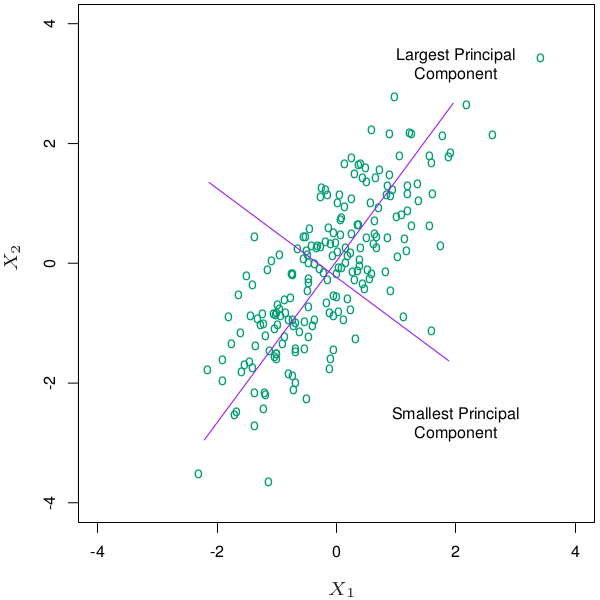
\includegraphics[width=0.69\textwidth]{pc}
}



\frame{\frametitle{Principal Component Regression: }
\framesubtitle{principal components}
Principal component regression (PCR):
\begin{itemize}
\item use $M\leq p$ principal components as \textcolor{uio}{input};
\item regress $y$ on $z_1, \dots, z_M$;
\item since the \textcolor{uio}{principal components} are \textcolor{uio}{orthogonal},
$$
\hat{y}_\text{pcr}(M) = \bar{y} + \sum_{m=1}^M \hat{\theta}_m z_m,
$$
where $\hat{\theta}_m = \langle z_m, y\rangle / \langle z_m, z_m \rangle$.
\end{itemize}
Since $z_m$ are linear combinations of $x_j$,
$$
\hat{\beta}_\text{pcr}(M) = \sum_{m=1}^M \hat{\theta}_m v_m.
$$
}


\frame{\frametitle{Principal Component Regression: }
\framesubtitle{remarks}
Note that:
\begin{itemize}
\item PCR can be used in \textcolor{uio}{high-dimensions}, as long as $M<n$;
\item idea: \textcolor{uio}{remove} the directions with \textcolor{uio}{less} information;
\item if $M=N$, $\hat{\beta}_\text{pcr}(M) = \hat{\beta}_\text{OLS}$;
\item $M$ is a \textcolor{uio}{tuning parameter}, may be chosen via cross-validation;
\item \textcolor{uio}{shrinkage effect} (clearer later);
\item[]
\item principal component are scale dependent, it is \textcolor{uio}{important to standardize} $X$!
\end{itemize}
}




\subsection{Partial Least Squares}

\frame{\frametitle{Partial Least Squares: }
\framesubtitle{idea}
Partial least square (PLS) is based on an idea \textcolor{uio}{similar} to PCR:
\begin{itemize}
\item construct a set of linear combinations of $X$;
\item \textcolor{uio}{PCR} only uses $X$, \textcolor{uio}{ignoring} $y$;
\item in PLS we want to \textcolor{uio}{also} consider the information on $y$;
\item as for PCR, it is important to \textcolor{uio}{first standardize} $X$.
\end{itemize}
}

\frame{\frametitle{Partial Least Squares: }
\framesubtitle{algorithm}
\begin{enumerate}
  \item standardize each $x_j$, set $\hat{y}^{[0]} = \bar{y}$ and $x_j^{[0]} = x_j$;
  \item For $m = 1, 2, \dots, p$,
  \begin{itemize}
    \item[(a)] $z_m = \sum_{j=1}^p \hat{\varphi}_{mj}x_j^{[m-1]}$, with $\hat{\varphi}_{mj} = \langle x_j^{[m-1]}, y \rangle$;
    \item[(b)] $\hat{\theta}_m = \langle z_m, y \rangle / \langle z_m, z_m \rangle$;
    \item[(c)] $\hat{y}^{[m]} = \hat{y}^{[m-1]} + \hat{\theta}z_m$;
    \item[(d)] orthogonalize each $x_j^{[m-1]}$ with respect to $z_m$,
    $$
    x_j^{[m]} = x_j^{[m-1]} - \left(\frac{\langle z_m, x_j^{[m-1]} \rangle}{\langle z_m, z_m \rangle}\right)z_m,\;\;\; j = 1, \dots, p;
    $$
  \end{itemize}
  \item output the sequence of fitted vectors $\{\hat{y}^{[m]}\}_1^p$.
\end{enumerate}
}


\frame{\frametitle{Partial Least Squares: }
\framesubtitle{step by step}
First step:
\begin{itemize}
\item[(a)] compute the \textcolor{uio}{first PLS direction}, $z_1 = \sum_{j=1}^p \hat{\varphi}_{1j}x_j$,
\begin{itemize}
\item based on the \textcolor{uio}{relation between each $x_j$ and $y$}, $\hat{\varphi}_1=\langle x_j, y \rangle$;
\end{itemize}
\item[(b)] estimate the related \textcolor{uio}{regression coefficient}, $\hat{\theta}_1 = \frac{\langle z_1, y \rangle}{\langle z_1, z_1 \rangle}=\frac{\widebar{z_1y}}{\widebar{z_1^2}}$;
\item[(c)] model after the first iteration: $\hat{y}^{[1]} = \bar{y} + \hat{\theta}_1z_1$;
\item[(d)] \textcolor{uio}{orthogonalize} $x_1,\dots,x_p$ w.r.t.\ $z_1$, $x_j^{[2]} = x_j - \left( \frac{\langle z_1, x_j \rangle}{\langle z_1, z_1 \rangle}\right)z_1$;
\end{itemize}
We are now ready for the second step \dots
}


\frame{\frametitle{Partial Least Squares: }
\framesubtitle{step by step}
\dots using $x_j^{[2]}$ instead of $x_j$:
\begin{itemize}
\item[(a)] compute the \textcolor{uio}{second} PLS direction, $z_2 = \sum_{j=1}^p \hat{\varphi}_{2j}x_j^{[2]}$,
\begin{itemize}
\item based on the relation between each \textcolor{uio}{$x_j^{[2]}$} and $y$, $\hat{\varphi}_2=\langle x_j^{[2]}, y \rangle$;
\end{itemize}
\item[(b)] estimate the related regression coefficient, $\hat{\theta}_2 = \frac{\langle z_2, y \rangle}{\langle z_2, z_2 \rangle}$;
\item[(c)] model after the second iteration: $\hat{y}^{[2]} = \bar{y} + \hat{\theta}_1z_1 + \hat{\theta}_2z_2$;
\item[(d)] orthogonalize $x_1^{[2]},\dots,x_p^{[2]}$ w.r.t.\ $z_2$, $x_j^{[2]} = x_j^{[2]} - \left( \frac{\langle z_2, x_j^{[2]} \rangle}{\langle z_2, z_2 \rangle}\right)z_2$;
\end{itemize}
and so on, \textcolor{uio}{until the $M\leq p$ step} $\rightarrow$ $M$ derived inputs.
}


\frame{\frametitle{Partial Least Squares: }
\framesubtitle{PLS versus PCR}
Differences:
\begin{itemize}
\item[PCR] the \textcolor{uio}{derived input directions} are the \textcolor{uio}{principal components} of $X$, constructed by looking at the variability of $X$;
\item[PLS] the input directions take into consideration \textcolor{uio}{both} the \textcolor{uio}{variability} of $X$ and the \textcolor{uio}{correlation} between $X$ and $y$.
\end{itemize}

\vspace{6pt}

Mathematically:
\begin{itemize}
\item[PCR] $\text{max}_\alpha \text{Var}(X\alpha)$, s.t.
\begin{itemize}
\item $||\alpha||=1$ and $\alpha^T S v_\ell=0$, $\ell = 1, \dots, M-1$;
\end{itemize} 
\item[PLS] $\text{max}_\alpha \text{Cor}^2(y,X\alpha)\text{Var}(X\alpha)$, s.t.
\begin{itemize}
\item $||\alpha||=1$ and $\alpha^T S \varphi_\ell=0$, $\forall \ell < M$.
\end{itemize}
\end{itemize}

\vspace{6pt}

In practice, the \textcolor{uio}{variance tends to dominate} $\rightarrow$ similar results!}



\section{Shrinkage Methods}

\subsection{Ridge Regression}

\frame{\frametitle{Ridge Regression: }
\framesubtitle{historical notes}
When two predictors are \textcolor{uio}{strongly correlated} $\rightarrow$ \textcolor{uio}{collinearity};
\begin{itemize}
\item in the extreme case of \textcolor{uio}{linear dependency} $\rightarrow$ \textcolor{uio}{super-collinearity};
\item in the case of super-collinearity, $X^TX$ is \textcolor{uio}{not invertible} (not full rank);
\end{itemize}

\hspace{2pt}

\cite{HoerlKennard1970}: $X^TX$ $\rightarrow$ $X^TX + \lambda I_p$, where $\lambda > 0$ and 
$$
I_p = \left(\begin{array}{cccc}
       1 & 0 & \dots & 0 \\
       0 & 1 & \dots & 0 \\
       \vdots & \vdots & \ddots & \vdots \\
       0 & 0 & \dots & 1
      \end{array}\right).
$$
With $\lambda>0$, $(X^TX + \lambda I_p)^{-1}$ exists.
}

\frame{\frametitle{Ridge Regression: }
\framesubtitle{estimator}
Substituting $X^TX$ with $X^TX + \lambda I_p$ in the LS estimator,
$$
\hat{\beta}_\text{ridge}(\lambda) = (X^TX + \lambda I_p)^{-1}X^Ty.
$$

Alternatively, the \textcolor{uio}{ridge estimator} can be seen as the \textcolor{uio}{minimizer} of
$$
\sum_{i = 1}^N (y_i - \beta_0 - \sum_{j=1}^p \beta_j x_{ij})^2,
$$
\textcolor{uio}{subject to} $\sum_{j=1}^p \beta_j^2 \leq t$.

\hspace{2pt}

Which is the same as
$$
\hat{\beta}_\text{ridge}(\lambda) = \text{argmin}_\beta \left\{\sum_{i = 1}^N (y_i - \beta_0 - \sum_{j=1}^p \beta_j x_{ij})^2 + \lambda \sum_{j=1}^p \beta_j^2\right\}.
$$
}


\frame{\frametitle{Ridge Regression: }
\framesubtitle{visually}
\centering
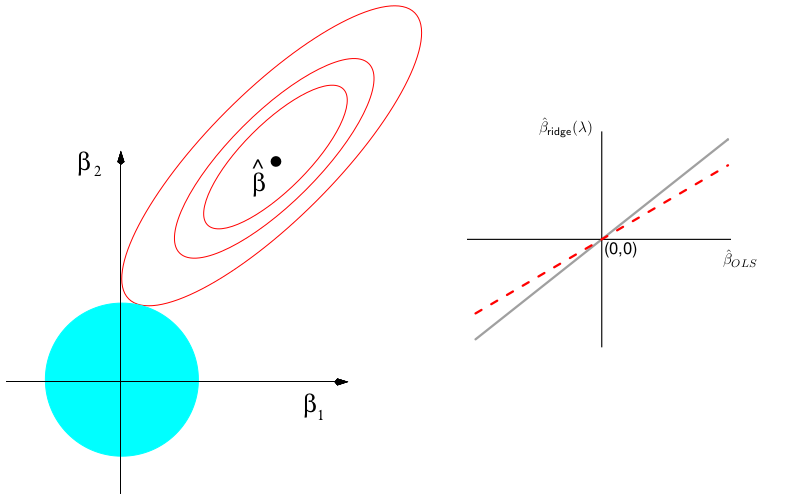
\includegraphics[width=\textwidth]{ridge_con}
}


\frame{\frametitle{Ridge Regression: }
\framesubtitle{visually}
\centering
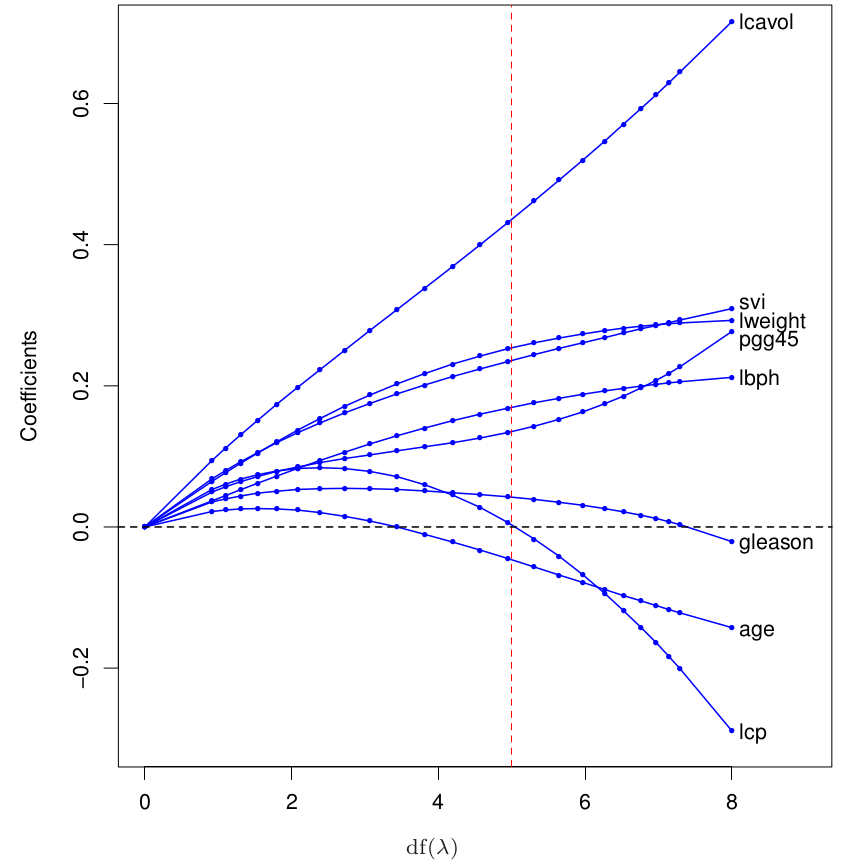
\includegraphics[width=0.7\textwidth]{ridge}
}


\frame{\frametitle{Ridge Regression: }
\framesubtitle{remarks}
Note:
\begin{itemize}
\item ridge solution is \textcolor{uio}{not equivariant under scaling} $\rightarrow$ $X$ must be \textcolor{uio}{standardized} before applying the minimizer;
\item the intercept is \textcolor{uio}{not involved} in the penalization;
\item[]
\item Bayesian interpretation:
\begin{itemize}
\item $Y_i \sim N(\beta_0 + x_i^T\beta, \sigma^2)$;
\item $\beta \sim N(0,\tau^2)$;
\item $\lambda = \sigma^2 / \tau^2$;
\item $\hat{\beta}_\text{ridge}(\lambda)$ as the posterior mean.
\end{itemize}
\end{itemize}
}


\frame{\frametitle{Ridge Regression: }
\framesubtitle{bias}
\begin{align*}
E[\hat{\beta}_\text{ridge}(\lambda)] &= E[(X^TX + \lambda I_p)^{-1}X^Ty]\\
  &= E[(I_p + \lambda (X^TX)^{-1})^{-1}\underbrace{(X^TX)^{-1}X^Ty}_{\hat{\beta}_\text{LS}}]\\
  &= \underbrace{(I_p + \lambda (X^TX)^{-1})^{-1}}_{w_\lambda}E[\hat{\beta}_\text{LS}]\\
  &= w_\lambda \beta \implies E[\hat{\beta}_\text{ridge}(\lambda)] \neq \beta \text{ for } \lambda>0.
\end{align*}
\begin{itemize}
\item $\lambda \rightarrow 0$, $E[\hat{\beta}_\text{ridge}(\lambda)] \rightarrow \beta$;
\item $\lambda \rightarrow \infty$, $E[\hat{\beta}_\text{ridge}(\lambda)] \rightarrow 0$ (without intercept);
\item due to correlation, $\lambda_a > \lambda_b \nRightarrow  |\hat{\beta}_\text{ridge}(\lambda)| > |\hat{\beta}_\text{ridge}(\lambda)|$.
\end{itemize}
}


\frame{\frametitle{Ridge Regression: }
\framesubtitle{variance}
Consider the variance of the ridge estimator,
\begin{align*}
\text{Var}[\hat{\beta}_\text{ridge}(\lambda)] &= \text{Var}[w_\lambda\hat{\beta}_\text{LS}]\\
  &= w_\lambda \text{Var}[\hat{\beta}_\text{LS}] w_\lambda^T \\
  &= \sigma^2 w_\lambda (X^TX)^{-1} w_\lambda^T.
\end{align*}
Then,
\small
\begin{align*}
&\text{Var}[\hat{\beta}_\text{LS}] - \text{Var}[\hat{\beta}_\text{ridge}(\lambda)] = \sigma^2 \left[(X^TX)^{-1} - w_\lambda (X^TX)^{-1} w_\lambda^T \right]\\
&\;\,= \sigma^2 w_\lambda \left[(I_p + \lambda (X^TX)^{-1})(X^TX)^{-1}(I_p + \lambda (X^TX)^{-1})^T - (X^TX)^{-1} \right]w_\lambda^T\\
&\;\,= \sigma^2 w_\lambda \left[((X^TX)^{-1} + 2\lambda (X^TX)^{-2} + \lambda^2 (X^TX)^{-3}) - (X^TX)^{-1} \right]w_\lambda^T\\
&\;\,= \sigma^2 w_\lambda \left[2\lambda (X^TX)^{-2} + \lambda^2 (X^TX)^{-3})\right]w_\lambda^T > 0
\end{align*}

\vspace{-8pt}

(since all terms are quadratic and therefore positive)
$$
\implies \text{Var}[\hat{\beta}_\text{ridge}(\lambda)] \preceq \text{Var}[\hat{\beta}_\text{LS}]
$$
}


\frame{\frametitle{Ridge Regression: }
\framesubtitle{degrees of freedom}
Note that the ridge solution is a \textcolor{uio}{linear combination} of $y$, as the least squares one:
\begin{itemize}
\item $\hat{y}_\text{LS} = \underbrace{X(X^TX)^{-1}X^T}_{H}y$ $\longrightarrow$ $df = \text{trace}(H) = p$;
\item $\hat{y}_\text{ridge} = \underbrace{X(X^TX + \lambda I_p)^{-1}X^T}_{H_\lambda}y$  $\longrightarrow$ $df(\lambda) = \text{trace}(H_\lambda)$;
\begin{itemize}
  \item $\text{trace}(H_\lambda) = \sum_{i=1}^p \frac{d_j^2}{d_j^2+\lambda}$;
  \item $d_j$ is the diagonal element of $D$ in the SVD of $X$;
  \item $\lambda \rightarrow 0$, $df(\lambda) \rightarrow p$;
  \item $\lambda \rightarrow \infty$, $df(\lambda) \rightarrow 0$.
\end{itemize}
\end{itemize}
}


\frame{\frametitle{Ridge Regression: }
\framesubtitle{more about shrinkage}
Recall the SVD decomposition $X=UDV^T$, and the properties
$$
U^TU = I_p = V^TV.
$$
\begin{columns}
\begin{column}{0.5\textwidth}
\begin{align*}
\hat{\beta}_\text{LS} &= (X^TX)^{-1}X^Ty\\
  &= (VDU^TUDV^T)^{-1}VDU^Ty \\
  &= (VD^2V^T)^{-1}VDU^Ty \\
  &= VD^{-2}V^TVDU^Ty \\
  &= VD^{-2}DU^Ty 
\end{align*}
\end{column}
\begin{column}{0.5\textwidth}
\vspace{-20pt}
\begin{align*}
\hat{y}_\text{LS} &= X\hat{\beta}_\text{LS}\\
  &= UDV^TVD^{-2}DU^Ty \\
  &= UDD^{-2}DU^Ty \\
  &= UU^Ty
\end{align*}
\end{column}
\end{columns}
}


\frame{\frametitle{Ridge Regression: }
\framesubtitle{more about shrinkage}
\begin{columns}
\begin{column}{0.5\textwidth}
\vspace{-36pt}
\begin{align*}
\hat{\beta}_\text{ridge} &= (X^TX+\lambda I_p)^{-1}X^Ty\\
  &= (VDU^TUDV^T+\lambda I_p)^{-1}VDU^Ty \\
  &= (VD^2V^T+\lambda VV^T)^{-1}VDU^Ty \\
  &= V(D^2+\lambda I_p)^{-1}V^TVDU^Ty \\
  &= V(D^2+\lambda I_p)^{-1}U^Ty 
\end{align*}
\end{column}
\begin{column}{0.5\textwidth}
\begin{align*}
\hat{y}_\text{ridge} &= X\hat{\beta}_\text{ridge}\\
  =& UDV^TV(D^2+\lambda I_p)^{-1}U^Ty \\
  =& UV^TVD^2(D^2+\lambda I_p)^{-1}U^Ty \\
  =& U \underbrace{D^2(D^2+\lambda I_p)^{-1}}_{\DownArrow[20pt][>=latex,ultra thick]}U^Ty
\end{align*}
\vspace{-16pt}
$$
\sum_{j=1}^p \frac{d_j^2}{d_j^2+\lambda}
$$
\end{column}
\end{columns}

So:
\begin{itemize}
\item \textcolor{uio}{small} singular values $d_j$ correspond to directions of the column space of $X$ with \textcolor{uio}{low} variance;
\item ridge regression \textcolor{uio}{penalizes the most} these directions.
\end{itemize}
}


\frame{\frametitle{Ridge Regression: }
\framesubtitle{more about shrinkage}
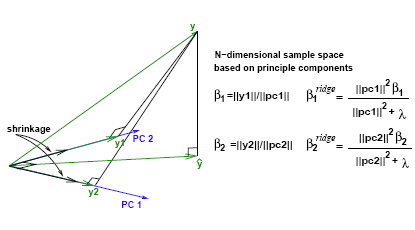
\includegraphics[width=\textwidth]{ridge_pc_down}
\scriptsize

(picture from \url{https://onlinecourses.science.psu.edu/stat857/node/155/})
}



%%%%%%%%%%%
\section*{Bibliography}
%%%%%%%%%%%

\frame[allowframebreaks]{\frametitle{References}
\footnotesize
\bibliographystyle{../../../../support/biometrika}
\bibliography{../../../../support/biblio}
}

\end{document}
